\documentclass{article} % Starts an article
\usepackage{tikz}
\usetikzlibrary{shapes.geometric, arrows, calc}
\usepackage[numbib]{tocbibind}
\tikzstyle{cool} = [rectangle, rounded corners, minimum width=3cm, minimum
height=1cm, text centered, draw=black, fill=gray!30, text width=3cm]
\tikzstyle{arrow} = [thick, ->, >=stealth]
\tikzstyle{line} = [thick, -, >=stealth]


\begin{document}



\tikzstyle{cool} = [rectangle, rounded corners, minimum width=3cm, minimum
height=1cm, text centered, draw=black, fill=gray!30, text width=3cm]
\tikzstyle{arrow} = [thick, ->, >=stealth]
\tikzstyle{line} = [thick, -, >=stealth]

\begin{figure}
    \centering
    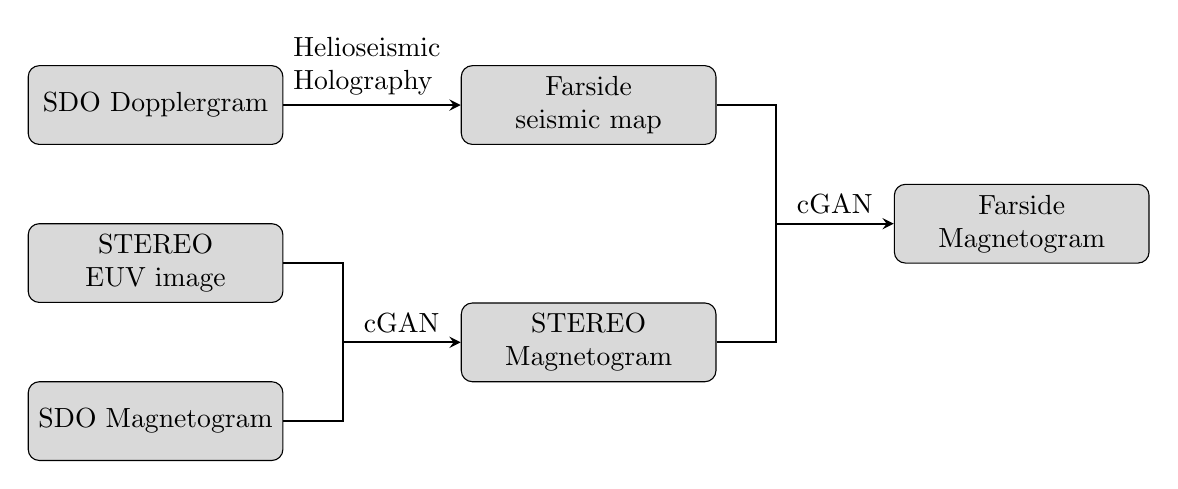
\begin{tikzpicture}[node distance=5.5cm]
        % \draw[help lines] (0,-5) grid (10,10);
        \node (D) [cool, above=1.5cm] {SDO Dopplergram};
        \node (P) [cool, right of=D] {Farside \quad \quad \quad \qquad  seismic map};
        \node (E) [cool] {STEREO EUV image};
        \node (M) [cool, right of=E, below=0.5cm] {STEREO Magnetogram};
        \node (F) [cool, right of=M, above=1cm] {Farside\\ Magnetogram};
        \node (S) [cool, below=1.5cm] {SDO Magnetogram};

        \coordinate (FF) at ([xshift=-1.5cm]F.west); % we collect the edges in front of Q
        \coordinate (MM) at ([xshift=-1.5cm]M.west); % we collect the edges in front of Q
        
        \draw [arrow] (D) -- node[anchor=south, text width=2cm] {Helioseismic Holography} (P);
        \draw [arrow] (MM) -- node[anchor=south] {cGAN} (M);
        \draw [line] (P) -|  (FF);
        \draw [line] (M) -|  (FF);
        \draw [line] (S) -|  (MM);
        \draw [line] (E) -|  (MM);
        \draw [arrow] (FF) -- node[anchor=south] {cGAN} (F);

    \end{tikzpicture}
    \caption{Test}
\end{figure}


\end{document}
